\documentclass{article} % For LaTeX2e
% \documentstyle[nips14submit_09,times,art10]{article} % For LaTeX 
\usepackage{nips15submit_e,times}
% \usepackage{nips_2017,times}
%\usepackage{hyperref}
%\usepackage{url}
% \usepackage[margin=1in]{geometry}

\usepackage{amsmath,amsthm,amssymb}
\usepackage{subcaption,graphicx}
\usepackage{tabularx}
\usepackage{float}
\usepackage{tabularx}
\newcommand{\N}{\mathbb{N}}
\newcommand{\Z}{\mathbb{Z}}
% 2.09

\title{Sentence Representations Models For Semantic Textual Similarity Task - A Comparsion Study}

% The \author macro works with any number of authors. There are two commands
% used to separate the names and addresses of multiple authors: \And and \AND.
%
% Using \And between authors leaves it to \LaTeX{} to determine where to break
% the lines. Using \AND forces a linebreak at that point. So, if \LaTeX{}
% puts 3 of 4 authors names on the first line, and the last on the second
% line, try using \AND instead of \And before the third author name.

\newcommand{\fix}{\marginpar{FIX}}
\newcommand{\new}{\marginpar{NEW}}

%\nipsfinalcopy % Uncomment for camera-ready version

\begin{document}


\maketitle


\begin{abstract}
Semantic similarity between two sentences is a basic language understanding problem that is applicable in many natural language processing applications. We replicated and extended existing works proposed in Association of Computer Linguistics' SemEval competitions to evaluate semantic models. We gathered features such as the length, vector spaces and text difference and implemented three models: SVM, RF, and CNN to measure semantic textual similarity. 
\end{abstract}

\section{Introduction}
Need for analysis of raw text has 
In last five years, there has been a tremendous increase in the research on estimating the similarity between two sentence.News headlines, sms and emails, tweets, image captions—the use of short text is
extensive, spanning a variety of domains and applications. Analysis of such raw textual data
can reveal information that is important, even critical, in different areas of modern human
life: education, security, business, law, healthcare, and so forth. Unsurprisingly, processing of
short text—sentences for example—is a primary focus in classical and contemporary natural
language processing (nlp).	`																		

\subsection{Semantic Textual Similarity (STS)}
\subsection{Applications of STS}
\subsection{Research Contributions}
\subsection{Contributions}
\section{Related Work}
\section

Research on estimating the semantic similarity between two sentence has been increasing in past five years. It applies to machine translation, question answering, and semantic text search etc. In distributional semantic models(DSM), the meaning of the words representations are approximated under a distributional vector space using the patterns of word co-occurring with other words in the corpus. DSMs are insubstantial in modeling the sentence representations because it does not capture the grammatical and syntactical aspect \cite{semeval2017}. Through this project, we will replicate and extend some of the existing works \cite{ecnu,CNN} mentioned below to get a better understanding of these models.
	

\subsection{Task Description}
	The task of semantic textual similarity involves two sub-task: 1)Sentence Relatedness, 2) Sentence Entailment. This project predicts the sentence relatedness for a given sentence pair. Normally for predicting the measure of textual similarity, we are given N list of sentence pair ($S_{ai},S_{bi}$)= \{($S_{a1},S_{b2}$),.., ($S_{aN},S_{bN}$)\}. The sentence pair comes with the similarity score \{$Y_{ab1}, Y_{ab2},...., Y_{abN}$\} that takes a value ranging from 0 indicating no similarity to 5 indicating the high similarity between the sentences. The goal is to build a model that for each sentence pair \textbf($S_{ai},S_{bi}$) generates an optimal similarity score \{$Y_{ab}$\} such that relevant sentence pair get high score. 
	
	Formally, the task is to learn
	
	\begin{align*} 
	h(w,f(S_a,S_b))  & \rightarrow Y_{ab} , \\
	\end{align*}
	
	where function f(·) maps sentence pairs to a features or a vector
	representation where each component expresses a certain type of
	similarity, e.g., lexical, syntactic, and semantic. The weight vector
	w is a parameter of the model that is learned during the training.
		
		For training and test of the STS model, we used data published in SemEval 2012-SemEval 2017 which includes the collection of STS dataset created using corpus from various domains like News headlines from the RSS feed of the European Media Monitor, Image captions from Flickr, Pairs of answers collected from Stack Exchange, student answers paired with correct reference answers from the BEETLE corpus, and Forum discussions about beliefs from the DEFT Committed Belief Annotation dataset \cite{sem-eval2105}. The performance of the model is measured using Pearson correlation of the predicted score with the human judgment score given in the dataset.

\section{Related Work}
	In 2012, supervised models based on the lexical and syntactic features of the sentence pair showed promising results on measuring semantic relatedness. These systems gave 52\% - 59\% correlation on various datasets by using regression models consisting of various similarity measure as its input features. Later, the unsupervised models did well for next two year in row using the WordNet knowledge and the LSA similarity measures which assume that the words with closer meaning highly co-occur in the text corpora. \cite{Align-Han2013} proposed three approaches that involved LSA similarity model, semantic similarity model based on the alignments quality of the sentences and support vector regression model that had features from different combination of similarity measures and the measures from other two core models.It is observed that using n-gram overlap feature increased LSA similarity model. Out of three models proposed \cite{Align-Han2013}, alignment based system  gave 59\%- 74.6\% pearson correlation on four different dataset. Using this model's alignment quality as one of the feature in the Support Vector Regression model improved the correlation score to 78 \%.  Various supervised models using unigram/bigram overlap, vector distance, and cosine similarity of sentence embedding were proposed \cite{sem-eval2105}. 
	
	Although using hand-crafted features with above mentioned models perform well, it has some drawbacks like tuning the features extracted on addressing the corpus from new domains, etc. Recent approaches in deep learning continues to prove the problem of semantic text matching can be  handled in a efficient way \cite{CNN, CNN-rank}. The problem of distributional word match can be generalized to the problem of the distributional sentence match by using deep learning approaches. This helps in effectively learning the individual meanings from embedding of all the words in the sentence and derives a meaningful sentence representation from the word vectors.
	
	In this project, we will implement three different models namely SVM, Random Forest and Convolutional Neural Network that measures the semantic similarity of a monolingual sentence pair. Our objective is to analyse the performance of each model and how the handcrafted features influences the Pearson correlation score. In CNN, the importance of the hyper-parameters are analyzed by tuning and comparing the change in the Pearson score.




	
	\section{Approach}
%	\subsection{Feature Engineering}
	In this section, we will discuss the models that we are exploring. We implemented the models proposed in \cite{CNN,ecnu} and further extended them and measured their performance using Pearson's Correlation.
	\subsection{Deep Learning Model}
		This section explains the deep learning model used for semantic sentence similarity. The two main components of this model are convolution neural networks(CNN) based sentence representation model and fully connected neural networks(FCNN) used as the multi-class classifier. The CNN architecture consists of two convolution networks that work in parallel to mapping the two sentences to a vector space. The distributional vectors of the sentence pairs are used by FCNN to classify its sentence similarity score. In the following, we first describe our sentence model for mapping sentence pair to their intermediate representations and then explain how these representations are used to classify the relatedness score.
	
	\subsubsection{Sentence Model using CNN}
	Our CNN architecture for mapping sentences to feature
	vectors inspired from \cite{CNN} is shown on Figure 1 . This architecture consists of two 1-dimensional convolution layer and a max pooling layer. The objective of this network is to convert the raw sentence into vector representations from \cite{glove}, pre-trained 300 dimension word embeddings of all the words \{$w_{1}, w_{2},...,w_{|s|}$\} present in the sentence.
	
	The input sentence to the convolution layers is treated as a sequence of real valued number where the real valued integers are retired from the integer-word mapping present in the vocabulary V. The vector representaion of all the word $ w \in \mathbb{R}^{d}  $ drawn from embedding matrix  $ W \in \mathbb{R}^{d \times |V|} $ in the embedding layer. To enhance the word representation with respect to this task, a true flag for word overlap is added as a additional dimension into the word vector representation for each word in the sentence. Then the CNN network applies convolution and max pooling operation to find the optimal feature vectos for the sentence that capture its semantics. 
	
	The idea behind the convolution layer is to learn the features which identifies the relationship between n-gram of the sentence using weight vectors \textit{m} $\in \mathbb{R}^{|m|}$ . The $1 \times 1$ weight vector \textit{m} also known as filters of the convolution is used. This convolution operation is followed by applying Relu activation function to learn non-linear decision boundaries. This filters out the insignificant features learnt in previous operation. The output from convolution layer is passed to max pooling layer with pool size (1, $|S|$) where the semantic information learnt is aggregated and reduuces representation dimension from $1 \times |S| \times 300$(word vec dimension) to $1 \times 300$(word vec dimension).The convolution layers along with Relu activation function and max pooling acts as non linear  feature detector for the given sentence. The output sentence representation from CNN is used to find Semantic Difference Matrix by performing a series of operation on the two sentence vector. 
	
	\begin{figure}[!tbp]
		\centering
		\begin{minipage}[b]{0.43\textwidth}
		\centering
		\label{CNN_1}
		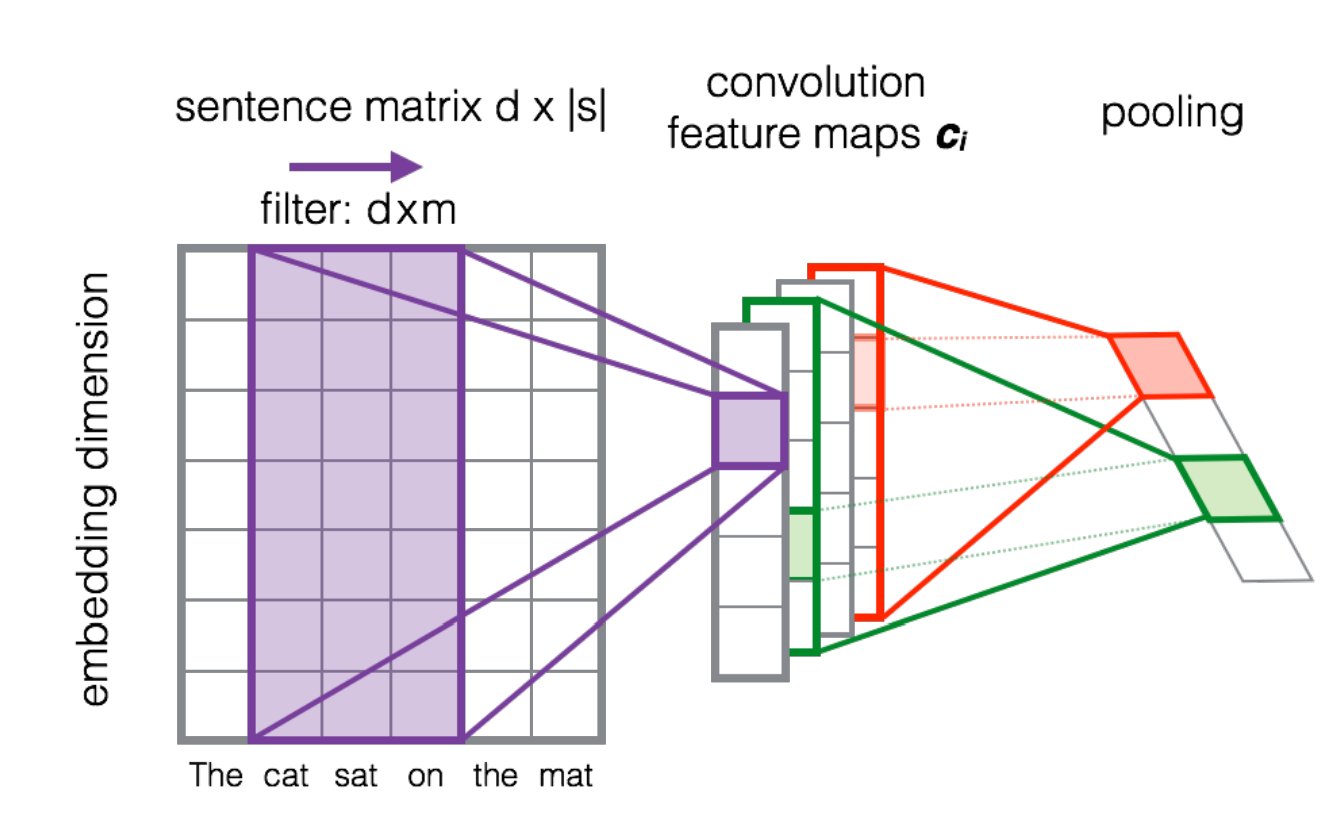
\includegraphics[scale=0.20]{CNN_sentModel.png}
		\caption{CNN Sentence Model \cite{CNN-rank}}
		\end{minipage}
		\hfill
		\begin{minipage}[b]{0.3\textwidth}
		\centering
		\label{params}
		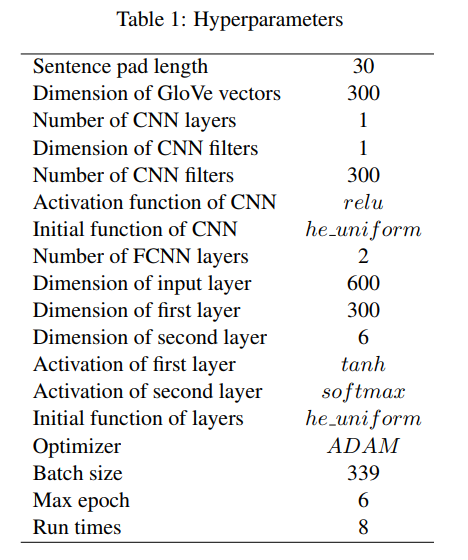
\includegraphics[scale=0.35]{hyperparameters.png}
		\caption{Hyperparameters for FCNN \cite{CNN}}
		\end{minipage}
	\end{figure}
	
	
	\subsubsection{Semantic Difference Matrix}
	The semantic difference matrix is generated by concatenating the vector difference and vector product of two sentence representation. This  matrix is used to classify the similarity measure using fully connected neural network(FCNN) with 2 dense layers. 
	
		\begin{align*} 
			SDV & =(|SV_{1}- SV_{2}|.(SV_{1} \circ SV_{2})) \\
		\end{align*}
	
	\subsubsection{Similarity Measure using FCNN}
	
	 This network consists of one hidden layer of size 300 nodes and a output layer of size 6.The hidden layer applies \textit{tanh} activation function and the output layer applies softmax layer. The softmax layer calculates the probability over the six score labels. The hyper parameters of this network is shown Figure \ref{params}
	 
	 Finally, the model is trained using the categorical cross-entropy loss: given a vector of probabilities p for a training pair of sentences, if the correct similarity category corresponds to index i of p, the model will evaluate the loss as $L = − log(pi)$.
	 

     	\subsection{Feature Extraction for SVM and RF}
		One test data row contains sentence A, sentence  B, and their level of similarity. Based on sentence A and B, we extracted the following features: cosine similarity, length, text difference, and knowledge-based similarity. We standardized the features to [-1, 1] via MinMaxScaler of sklearn.

\subsubsection{Preprocessing}
Before the feature extraction, we preprocessed data in three ways. We opened contractions to their formal writings. For example, 'doesn’t' was rewritten as 'does not'. WordNet-based Lemmatizer implemented in Natural Language Toolkit2 lemmatized all words to their nearest base forms. For example, 'was' was lemmatized to 'be'. Finally, we replaced a word from one sentence with another word from the other sentence if they were synonyms. WordNet's extensive word library effectively found the synonyms. Word sense disambiguation and synonym filtering on a particular lemma was out of this project's scope.
 
\subsubsection{Cosine Similarity}
 We calculated the distributional vector of each word in the same sentence and measured the cosine of the angle between two vector pairs \cite{gomaa}

\subsubsection{Length Features}
We measured the length of unique words in each sentences ($|A|$ and $|B|$), the length of their differences ($|A-B|, |B-A|, \frac{|A-B|}{|B|},  \frac{|B-A|}{|A|}$), the length of their intersection and union ($|A \cup B|$ and $|A \cap B| $). After that, we grouped words by their POS tags and found number different nouns in A but not in B. Same was repeated for verb, adjective and adverb.

\subsubsection{Knowledge-Based Similarity Measures}
We chose four semantic similarity measures in Wordnet: Jiang \& Conrath (jcn) \cite{jcn} which measures the information content and Leacock \& Chodorow (lch) \cite{lch}, Wu \& Palmer (wup) \cite{wup} and Path Length (path) \cite{path} which measure path length. jcn measures how similar two word senses were based on the Information Content (IC) of the Least Common Subsumer (LCS), which is the most informative subsumer connecting the two words senses together. For our test, we based the algorithm on the commonly used and effective Brown corpus \cite{liu}. path is the shortest path connecting the senses together in a is-a taxonomy. lch also measures the shortest path, but looks at the maximum depth of the taxonomy where the senses appear. Finally, wup measures the the depth of the taxonomy, but also measures the depth of their LCS. 

\subsubsection{Text Difference Measures}
If length feature looks at the number of similar words, text difference measures the number of contradicting words. Experiment in \cite{ecnu} measures contradiction as 1 if there is an antonym between two sentence pairs or if the negation status is not consistent and -1, otherwise. We extended the paper to open the single feature into three features: the number of A's antonym in B, the number of B's antonym in A, and the consistency of the number of negation words in both sentences. Next, we deleted the repeating words found in both sentence pairs and applied the same four similarity measures. We recorded the maximum, minimum, and average value of each measure to calculate STS when text pairs have words of similar meaning, but not the same spelling.

     	\subsubsection{SVM}
We trained the Support Vector Regression (SVR) to predict relatedness score based on our features. Support Vector Machine (SVM) and kernel methods was the most popular learning methods in SemEval-2015 Task 1 competition {SemEval2015} because it nicely separated multiple features into different dimensional space and made decisions according to the hyperplanes. We used NuSVR in the Scikit-learn toolkit which implements SVR, but with a parameter nu to control the number of support vectors. For this project, we compared radial basis function (RBF) kenels, polynomial kernels, and linear support vector regression to evalue which method can effectively use our features to accurately predict the relatedness score. \cite{Abualigah} used the default RBF kernel that is defined $K(a, b) = exp(\frac{ \parallel a-b \parallel ^2}{2 \sigma ^2})$. Here, the distance between two points measures their similarity. The polynomial kernel is another option that is more popular in natural language processing {poly}. It is defined as $K(a, b) = (a^Tb + c)^d$ for degree-d polynomials where c is a free parameter trading off the influence of different terms in the polynomial. Linear support vector regression separates our features linearly.

     	\subsubsection{RF}
We trained Random Forest model to predict relatedness score based on same features as SVN. Based on this features, Random Forest model constructed a multitude of decision tree at training time and selects the mode of the classes output by the individual trees. We used Random Forest Regressor from Scikit. With such simple algorithm, RF model reached over 0.77 Pearson correlation.

	\section{Experiments}
    
     	\subsection{Feature Extraction for SVM and RF}
Each feature groups, including cosine similarity, length feature, semantic similarity, and text difference, played crucial roles increasing the overall Pearson correlation coefficient. Cosine similarity measured the similarity between two sentences the best. Adding the length feature actually decreased the STS score in the paper that we based our project on \cite{ecnu}, but was proven to be an effective way of measuring semantic similarity of texts in \cite{corley}, so we experimented with this feature, and it raised our STS score. We experimented with different semantic similarity measures in Wordnet, but have found that combining the above four algorithms, jcn, lch, wup and path can most accurately predict the STS of our sentence pairs. The three separate text difference features, including the number of A's antonym in B, the number of B's antonym in A, and the consistency of the number of negation words in both sentences, increased our accuracy score. Combining them to one feature would have decreased the accuracy. Effective, individual features combined to create a better performance overall.

\begin{figure}[h]
\begin{center}
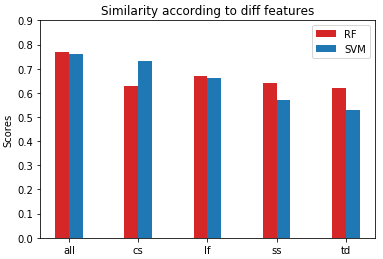
\includegraphics[scale=0.8]{Capture.PNG}
\end{center}
\caption{Result of feature combinations in SVM and RF}
\end{figure}

In SVM, RBF and polynomial kernel predicted the relatedness score more accurately than the linear kernel. Pearson correlation coefficient for SVR with RBF kernel, SVR with polynomial kenel, and linear SVR was 0.765, 0.762, and 0.513, repectively. Linear support vector regression was a poor method because our features could not be separately linearly. On the other hand, with the RBF and polynomial kernel, it did not need to be separately linearly.  

In RF, relatedness score was most accurate with 150 division trees, compared to 40 which was used in the \cite{ecnu} competition . In terms of features, among four of them, the model did significantly bad with cosine similarity feature. Other than cosine similarity measure, random forest model performed better than SVM model. This was also true with combination of all features.

	\subsection{Deep Learning Model from \cite{CNN}}
	 Intially, the model was trained using 4500 sentence pair (20 \% of the whole dataset from SemEval2012 - SemEval 2014) with the valdiation set of 500 sentence pair. The pearson correlation was used as evaluation metric for the model. The observed correlation was 78\% on training data and 36.6 \% on testing data after 10 epochs. Initially, 200000 word embeddings from Word2Vec without any enhancements were used. After loading all 3 million pre-trained word embeddings and increasing the training dataset size to 15457, the accuracy improved to 47.6 \% on test data. Initial accuracy was low because many words were treated as out of vocabulary words and those words were filtered out while learning the sentence representations.
	 \begin{figure}[htp]
  % Equal length
  \hspace*{\fill}%
  \subcaptionbox{Training and Validation Correlation\cite{CNN-rank}\label{CNN_acc}}{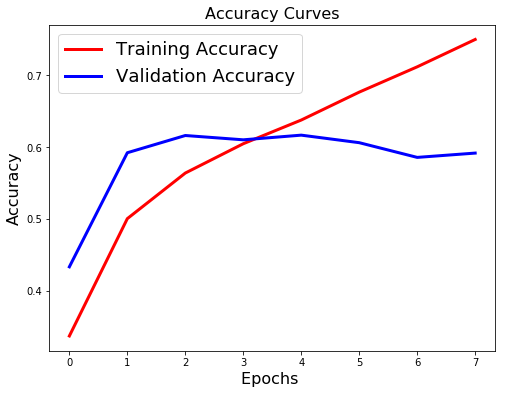
\includegraphics[width=2.0in]{graph1.png}}\hfill%
  \subcaptionbox{Training and Validation loss \cite{CNN}\label{CNN_loss}}{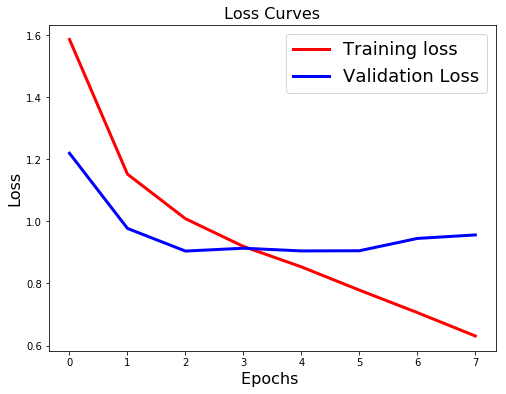
\includegraphics[width=2.0in]{graph2.png}}%
  \hspace*{\fill}%
\end{figure}

	 \subsubsection{Enhancing the word embedding}
	 We enhanced the input word vectors using hand crafted features \cite{CNN}. We added a True/False flag for every word specifying if that word was present in both the sentences. This improved the test correlation from 47\% to 54\% while the training correlation was around 86\%. This shows how the model was clearly overfitting on the train set. 
	 
	 \subsubsection{Adding deep network}
	 As the model presented in \cite{CNN} was overfitting, we experimented by adding more layers and adding regularizers. Adding just one Dense layer in FCNN improved the testing correlation by 2\% to 56\%. Further adding more layers in FCNN did not improve the correlation much but it achieved similar correlation with lesser epochs. As for the Convolution network, increasing the depth of the network did not result in improved performance. We found 2 layers at CNN and 3 layers at FCNN was optimal.
	 
	 \subsubsection{Adding regularization}
	 Although deep learning models can learn complex functions, they overfit the training data very easily when the size of the dataset is small \cite{CNN-rank}. To handle the overfitting issue, l2-norm regularization terms was added to the layer parameters of the network. After this, the the difference between training accuracy and testing correlation reduced and testing correlation improved to 59\%.
	 
	 \subsubsection{Adding more data}
	 To test the validity of the model for this task, we experimented it under more training data settings. Since 20000 pair of sentence was not enough data for neural network model to learn to generalize well, we added this experiment. For this experiment, we took data from one of the SemEval tasks for Question Answering which was very similar to the our original data. In this dataset, a pair of question and an answer are given a score from 0-5 on how possible that answer is for the question. The dataset size was 300000 sentence pair. Our model gave training correlation of 77\% and testing correlation of 72\% for 8 epochs. Since this training took a really long time we couldn't experiment for more epochs under different parameter. This shows that the model is well suited for this task when large dataset is provided.

	\section{Conclusion}
   We explored the effectiveness of Random Forest, Support Vector Machine and Convolutional Neural Netowrk model for task of measuring semantic similarity of two sentence using various features combined with pre-trained word vector representations. Based on same features (cosine similarity, length features, semantic similarity, and text difference), SVM and RF performed similarly, reaching up to 0.77 Pearson correlation measure in compare of original similarity measure. By reproducing the CNN models in \cite{CNN} with same hyperparameters, the model achieved 54 \% Pearson correlation. After tuning the parameters, the correlation of the model improved to 61 \%. On training this model with really large dataset, the accuracy improved to 72\%. Results of this CNN in the 2017 SemEval challenge achieved 81.56\%  for the monolingual sentence relatedness task. We conclude that using diverse handcrafted features for RF and SVM models improve the prediction. On the other hand, a simple neural network models without any handcrafted features is competitive with RF and SVM models provided large dataset. 
    	
\subsection*{Contributions}
\begin{enumerate}
\item \textbf{Lim}  preprocessed sentence pairs for Random Forest and SVM models and used Random Forest Model to get a good Pearson correlation.
\item \textbf{Joanne} selected and developed features for Random Forest and SVM models, and applied the features into the SVM algorithm.
\item \textbf{Aarthi} Literature Survey. Implementing neural network model with custom evaluation metric function. Experiments on CNN model. 
\end{enumerate}
 
\begin{thebibliography}{9}
	\bibitem{semeval2017} Agirre, E., Cer, D.M., Diab, M.T., Lopez-Gazpio, I., \& Specia, L. (2017). SemEval-2017 Task 1: Semantic Textual Similarity - Multilingual and Cross-lingual Focused Evaluation. {\it SemEval@ACL}.
	
	\bibitem{sem-eval2105}Agirre, E., Banea, C., Cardie, C., Cer, D.M., Diab, M.T., \&Gonzalez-Agirre, A.. (2015). SemEval-2015 Task 2: Semantic Textual Similarity, English, Spanish and Pilot on Interpretability.  {\it SemEval@NAACL-HLT}. 
        
    \bibitem{Align-Han2013} Finin, T.W., Han, L., Kashyap, A.L., Mayfield, J., \& Weese, J. (2013) UMBC\_EBIQUITY-CORE: Semantic Textual Similarity Systems. {\it SEM@NAACL-HLT.}

	\bibitem{CNN} Shao, Y. (2017). HCTI at SemEval-2017 Task 1: Use convolutional neural network to evaluate Semantic Textual Similarity. {\it SemEval@ACL}.
    
	\bibitem{CNN-rank}Severyn, A., \& Moschitti, A. (2015, August).\textit {Learning to rank short text pairs with convolutional deep neural networks.} In Proceedings of the 38th International ACM SIGIR Conference on Research and Development in Information Retrieval (pp. 373-382). ACM.
	
	\bibitem{glove} Goldberg, Y., \& Levy, O. (2014). word2vec Explained: deriving Mikolov et al.'s negative-sampling word-embedding method. arXiv preprint arXiv:1402.3722.
    
   \bibitem {gomaa} Fahmy, A.A.,\& Gomaa, W.H. (2013). A Survey of Text Similarity Approaches. {\it International Journal of Computer Applications}, 68, 13-.18
   
    \bibitem{jcn} Jiang, J. \& Conrath, D. (1997). Semantic similarity based on corpus statistics and lexical taxonomy. In Proceedings of the International Conference on Research in Computational Linguistics, Taiwan.
    
    \bibitem{lch} Leacock, C. \& Chodorow, M. (1998). Combining local context and WordNet similarity for word sense identification. In C. Fellfaum (ed.), {\it MIT Press} pp. 265--283, Cambridge, Massachusetts. 
    
    \bibitem{wup}  Wu, Z.\& Palmer, M. (1994). Verb semantics and lexical selection. In Proceedings of the 32nd Annual Meeting of the Association for Computational Linguistics, Las Cruces, New Mexico.
        
   \bibitem{path}  Rada, R., Mili, H., Bicknell, E., \& Blettner, M. (1989). Development and application of a metric on semantic nets. {\it Systems, Man and Cybernetics, IEEE Transactions on}, 19(1), 17-30.
    

   \bibitem{liu} Liu, Y., Lin, L., Sun, C., Wang, X., \& Zhao, Y. (2015). Computing Semantic Text Similarity Using Rich Features. {\it PACLIC}.
   
	\bibitem{ecnu} Lan, M., Zhao, J., \& Zhu, T. (2014). ECNU: One Stone Two Birds: Ensemble of Heterogenous Measures for Semantic Relatedness and Textual Entailment. {\it SemEval@COLING}. 
    
   \bibitem{Abualigah} Abualigah, L.M., Al-Betar, M.A., Alomari, O.A., \& Khader, A.T. (2017). Text feature selection with a robust weight scheme and dynamic dimension reduction to text document clustering. {\it Expert Syst. Appl., 84}, 24-36.
   
   \bibitem{corley} Corley, C., Mihalcea, R., \& Association For Computational Linguistics. (2005). Measuring the Semantic Similarity of Texts.
    
\end{thebibliography}
\end{document}